% Options for packages loaded elsewhere
\PassOptionsToPackage{unicode}{hyperref}
\PassOptionsToPackage{hyphens}{url}
%
\documentclass[
]{article}
\usepackage{lmodern}
\usepackage{amssymb,amsmath}
\usepackage{ifxetex,ifluatex}
\ifnum 0\ifxetex 1\fi\ifluatex 1\fi=0 % if pdftex
  \usepackage[T1]{fontenc}
  \usepackage[utf8]{inputenc}
  \usepackage{textcomp} % provide euro and other symbols
\else % if luatex or xetex
  \usepackage{unicode-math}
  \defaultfontfeatures{Scale=MatchLowercase}
  \defaultfontfeatures[\rmfamily]{Ligatures=TeX,Scale=1}
\fi
% Use upquote if available, for straight quotes in verbatim environments
\IfFileExists{upquote.sty}{\usepackage{upquote}}{}
\IfFileExists{microtype.sty}{% use microtype if available
  \usepackage[]{microtype}
  \UseMicrotypeSet[protrusion]{basicmath} % disable protrusion for tt fonts
}{}
\makeatletter
\@ifundefined{KOMAClassName}{% if non-KOMA class
  \IfFileExists{parskip.sty}{%
    \usepackage{parskip}
  }{% else
    \setlength{\parindent}{0pt}
    \setlength{\parskip}{6pt plus 2pt minus 1pt}}
}{% if KOMA class
  \KOMAoptions{parskip=half}}
\makeatother
\usepackage{xcolor}
\IfFileExists{xurl.sty}{\usepackage{xurl}}{} % add URL line breaks if available
\IfFileExists{bookmark.sty}{\usepackage{bookmark}}{\usepackage{hyperref}}
\hypersetup{
  hidelinks,
  pdfcreator={LaTeX via pandoc}}
\urlstyle{same} % disable monospaced font for URLs
\usepackage[paper=a4paper,lmargin=2cm, rmargin=2cm, tmargin=2cm, bmargin=2cm]{geometry}
\usepackage{longtable,booktabs}
% Correct order of tables after \paragraph or \subparagraph
\usepackage{etoolbox}
\makeatletter
\patchcmd\longtable{\par}{\if@noskipsec\mbox{}\fi\par}{}{}
\makeatother
% Allow footnotes in longtable head/foot
\IfFileExists{footnotehyper.sty}{\usepackage{footnotehyper}}{\usepackage{footnote}}
\makesavenoteenv{longtable}
\usepackage{graphicx}
\makeatletter
\def\maxwidth{\ifdim\Gin@nat@width>\linewidth\linewidth\else\Gin@nat@width\fi}
\def\maxheight{\ifdim\Gin@nat@height>\textheight\textheight\else\Gin@nat@height\fi}
\makeatother
% Scale images if necessary, so that they will not overflow the page
% margins by default, and it is still possible to overwrite the defaults
% using explicit options in \includegraphics[width, height, ...]{}
\setkeys{Gin}{width=\maxwidth,height=\maxheight,keepaspectratio}
% Set default figure placement to htbp
\makeatletter
\def\fps@figure{htbp}
\makeatother
\setlength{\emergencystretch}{3em} % prevent overfull lines
\providecommand{\tightlist}{%
  \setlength{\itemsep}{0pt}\setlength{\parskip}{0pt}}
\setcounter{secnumdepth}{5}
\usepackage[portuguese]{babel}
\usepackage[utf8]{inputenc}
\usepackage[T1]{fontenc}
\usepackage{amsthm,amssymb,amsfonts,amsmath}
\usepackage{bm}
\usepackage{setspace}
\usepackage{multirow}
\usepackage{booktabs}
\usepackage{graphicx}
\usepackage{enumerate}
\usepackage{times}
\usepackage{xcolor}
\usepackage{csquotes}
\usepackage{natbib}
\usepackage{xcolor}

\addto\captionsportuguese{
      \renewcommand{\contentsname}%
        {Sumário}%
  }
  
\newlength{\drop}


\newcommand{\HRule}{\rule{\linewidth}{0.5mm}}

\usepackage[all]{background}

\backgroundsetup{
placement=center,
scale=1.5,
color=black,
opacity=0.075,
angle=0,
contents={
  \includegraphics[width=0.65\linewidth]{logo-ufba}
  }
}

\DeclareMathOperator{\vari}{Var}
\DeclareMathOperator{\espe}{E}
\DeclareMathOperator*{\argmax}{arg\,max}
\DeclareMathOperator*{\argmin}{arg\,min}

% silence everypage latex package used by background package
\usepackage{silence}
\WarningsOff[everypage]% Suppress warnings related to package everypage
\newlength{\cslhangindent}
\setlength{\cslhangindent}{1.5em}
\newenvironment{cslreferences}%
  {\setlength{\parindent}{0pt}%
  \everypar{\setlength{\hangindent}{\cslhangindent}}\ignorespaces}%
  {\par}

\author{}
\date{\vspace{-2.5em}}

\begin{document}

\onehalfspacing

\begin{titlepage}
    \drop=0.1\textheight
    \centering
    \vspace*{\baselineskip}
    \rule{\textwidth}{1.6pt}\vspace*{-\baselineskip}\vspace*{2pt}
    \rule{\textwidth}{0.4pt}\\[\baselineskip]
    {\LARGE RELATÓRIO FINAL \\ 
    \vspace*{\baselineskip}
    VALIDAÇÃO DE ESCALA DE CONHECIMENTO, ATITUDES E PRÁTICAS DE PROFESSORES SOBRE O TRANSTORNO DO ESPECTRO AUTISTA -- FASE 2}\\[0.2\baselineskip]
    \rule{\textwidth}{0.4pt}\vspace*{-\baselineskip}\vspace{3.2pt}
    \rule{\textwidth}{1.6pt}\\[\baselineskip]
    \scshape
    Trabalho de consultoria realizado no contexto da ação de extensão da Universidade Federal da Bahia com título \textit{Consultoria Estatística}. \\
    \vspace*{2\baselineskip}
    Elaborado por \\[\baselineskip]
    {\Large Gilberto Pereira Sassi\par}
    \vfill
    {\scshape 2021} \\
    {\large Universidade Federal da Bahia}\\
    {\large Instituto de Matemática e Estatística}\\
    {\large Departamento de Estatística}\par
  \end{titlepage}

\newpage

\tableofcontents

\newpage

\hypertarget{introduuxe7uxe3o}{%
\section{Introdução}\label{introduuxe7uxe3o}}

Este relatório apresenta os resultados da análise estatística do conjunto de dados referente à seguinte consultoria:

\begin{itemize}
\tightlist
\item
  \textbf{Consulente:} Danilo de Assis Pereira;
\item
  \textbf{Título do projeto:} Validação de escala de conhecimento, atitudes e práticas de professores sobre transtorno do espectro autista.
\end{itemize}

\hypertarget{materiais-e-muxe9todos}{%
\section{Materiais e métodos}\label{materiais-e-muxe9todos}}

O consulente pediu apoio no sexto passo do polo teórico na validação de conteúdo da escala de \emph{conhecimento, atitude e prática } do modelo psicométrico proposto por Pasquali (\protect\hyperlink{ref-pasquali1999elaboraccao}{1999}). Nesta consultoria, construimos o Gráfico do Coeficiente de Validade de Conteúdo em relação à clareza/compreensão e relevância dos itens.

Todas as computações e gráficos foram construídas usando a linguagem \texttt{R} (R Core Team \protect\hyperlink{ref-Rlang}{2021}).

\hypertarget{cuxe1lculo-do-coeficiente-de-validade-de-conteuxfado}{%
\subsection{Cálculo do Coeficiente de Validade de Conteúdo}\label{cuxe1lculo-do-coeficiente-de-validade-de-conteuxfado}}

Primeiramente, eu usei a seguinte codificação para calcular o Coeficiente de Validade de Conteúdo (CVC) para a análise de \emph{clareza e compreensão}:

\begin{enumerate}
\def\labelenumi{\arabic{enumi}.}
\tightlist
\item
  \emph{nada claro} corresponde ao valor 1;
\item
  \emph{pouco claro} corresponde ao valor 2;
\item
  \emph{muito claro} corresponde ao valor 3;
\item
  \emph{totalmente claro} corresponde ao valor 4;
\end{enumerate}

E para a análise de \emph{relevância}, eu usei a seguinte codificação:

\begin{enumerate}
\def\labelenumi{\arabic{enumi}.}
\tightlist
\item
  \emph{nada relevante} corresponde ao valor 1;
\item
  \emph{pouco relevante} corresponde ao valor 2;
\item
  \emph{muito relevante} corresponde ao valor 3;
\item
  \emph{totalmente relevante} correspondeo ao valor 4.
\end{enumerate}

Para computar o Coeficinte de Validade Conteúdo para o item em um instrumento com \(I\) itens avaliado por \(J\) juízes, usamos o seguinte algoritmo:

\begin{enumerate}
\def\labelenumi{\arabic{enumi}.}
\tightlist
\item
  Calcular a nota média do item \(i\): \(\bar{x}_i = \frac{\sum_{j=1}^{J}x_j}{J}\);
\item
  Penalização de vieses dos juízes: \(P_i = \frac{1}{J}\);
\item
  Calcular o Coeficiente de Validade do Conteúdo do \(i\)-ésimo item: \(CVC_i = \frac{\bar{x}_i}{\max{\{x_1, \dots, x_J\}}} - P_i\);
\item
  Finalmente, o Coeficiente de Validade do instrumento é dado por: \(CVC_t = \frac{\sum_{i=1}^{I}CVC_i}{I}\).
\end{enumerate}

O instrumento do consulente tem \(I = 22\) itens e foram consultados \(J = 52\) juízes.

Todos os cálculos desta seção seguiram as instruções e orientações de Firmiano (\protect\hyperlink{ref-firmiano2017escala}{2017}) disponbilizadas pelo consulente.

\newpage

\hypertarget{resultados}{%
\section{Resultados}\label{resultados}}

Nesta seção, vou incluir os resultados preliminares obtidos.

\hypertarget{gruxe1fico-do-coeficiente-de-validade-de-conteuxfado-em-relauxe7uxe3o-uxe0-clarezacompreensuxe3o-e-relevuxe2ncia-dos-itens-primeira-versuxe3o}{%
\subsection{Gráfico do Coeficiente de Validade de Conteúdo em relação à clareza/compreensão e relevância dos itens (primeira versão)}\label{gruxe1fico-do-coeficiente-de-validade-de-conteuxfado-em-relauxe7uxe3o-uxe0-clarezacompreensuxe3o-e-relevuxe2ncia-dos-itens-primeira-versuxe3o}}

Na Figura \ref{fig:grafico2V1}, incluimos o gráfico com o coeficiente CVC de clareza/compreensão e com o coeficiente de CVC de relevância para cada item. Além disso, incluímos o valor de referência recomendando por Hernández-Nieto (\protect\hyperlink{ref-hernandez2002contributions}{2002}) que é \(0,98\). Esse valor é alto, e por isso sugiro usar \(75\%\) de \(\left(1 - \frac{1}{52}\right) \cdot 0,75 = 0,74\), ou seja, no gráfico da Figura \ref{fig:grafico2V1} usamos o valor de referência \(0,74\) no lugar do valor de referência \(0,98\).

\begin{figure}[htbp]

{\centering 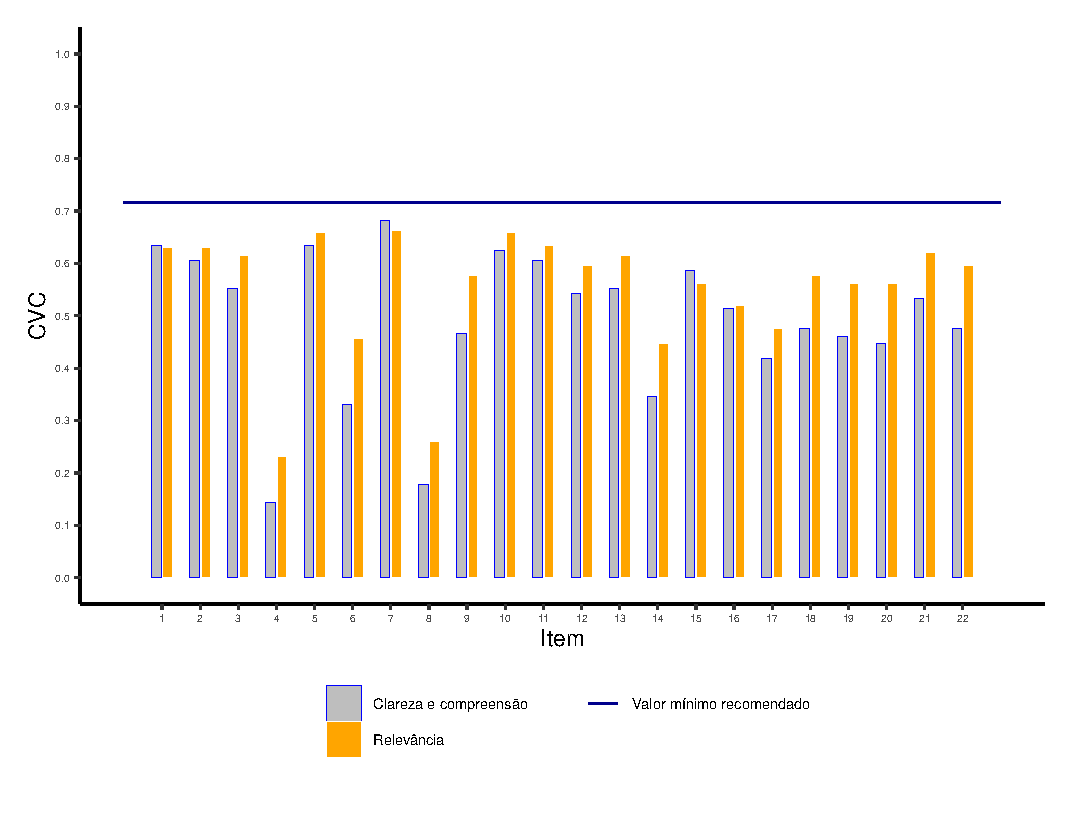
\includegraphics[width=0.9\linewidth]{../figures/grafico2_0_8} 

}

\caption{Gráfico de distribuição das características dos juízes.}\label{fig:grafico2V1}
\end{figure}

\newpage

\hypertarget{gruxe1fico-do-coeficiente-de-validade-de-conteuxfado-em-relauxe7uxe3o-uxe0-clarezacompreensuxe3o-e-relevuxe2ncia-dos-itens-segunda-versuxe3o}{%
\subsection{Gráfico do Coeficiente de Validade de Conteúdo em relação à clareza/compreensão e relevância dos itens (segunda versão)}\label{gruxe1fico-do-coeficiente-de-validade-de-conteuxfado-em-relauxe7uxe3o-uxe0-clarezacompreensuxe3o-e-relevuxe2ncia-dos-itens-segunda-versuxe3o}}

Na Figura \ref{fig:grafico2V2}, incluimos o gráfico com o coeficiente CVC de clareza/compreensão e com o coeficiente de CVC de relevância para cada item. Além disso, incluímos o valor de referência \(0,6\). Como a amostra tem 52 juízes, o valor máximo do coeficiente CVC é \(1-\frac{1}{52}\approx 0,98\) para esta amostra de juízes. Esse valor é alto, e por isso sugiro usar \(75\%\) de \(\left(1 - \frac{1}{52}\right) \cdot 0,75 = 0,74\), ou seja, no gráfico da Figura \ref{fig:grafico2V1} usamos o valor de referência \(0,74\) no lugar do valor de referência \(0,98\).

\begin{figure}[htbp]

{\centering 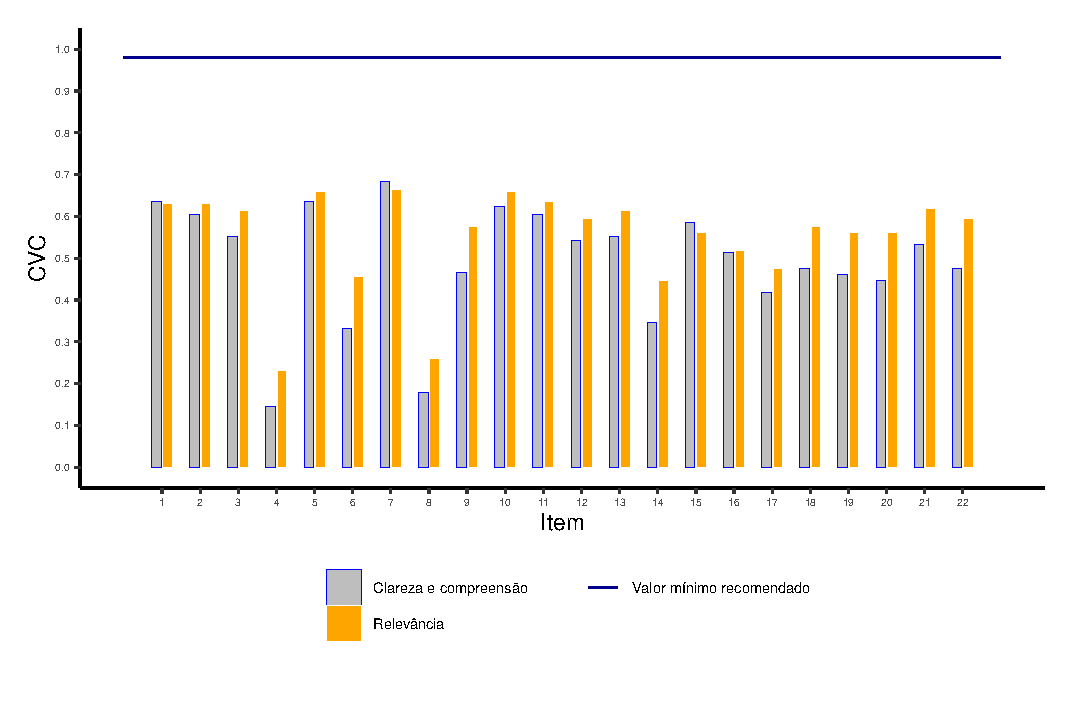
\includegraphics[width=0.9\linewidth]{../figures/grafico2_80_perc} 

}

\caption{Gráfico de distribuição das características dos juízes.}\label{fig:grafico2V2}
\end{figure}

\cleardoublepage

\hypertarget{referuxeancias}{%
\section*{Referências}\label{referuxeancias}}
\addcontentsline{toc}{section}{Referências}

\hypertarget{refs}{}
\begin{cslreferences}
\leavevmode\hypertarget{ref-firmiano2017escala}{}%
Firmiano, Maria Luisa Veras. 2017. ``Escala de Avaliação Do Conhecimento, Atitude E Prática de Gestantes Sobre Incontinência Urinária: Construção E Validação de Conteúdo.'' Master's thesis, Universidade Federal do Ceará.

\leavevmode\hypertarget{ref-hernandez2002contributions}{}%
Hernández-Nieto, Rafael A. 2002. ``Contributions to Statistical Analysis.'' \emph{Mérida: Universidad de Los Andes} 193.

\leavevmode\hypertarget{ref-pasquali1999elaboraccao}{}%
Pasquali, L. 1999. \emph{Elaboração de Instrumentos Psicológicos: Manual Prático de Elaboração}. LabPAM/IBAPP, Brasília, DF: IBAPP.

\leavevmode\hypertarget{ref-Rlang}{}%
R Core Team. 2021. \emph{R: A Language and Environment for Statistical Computing}. Vienna, Austria: R Foundation for Statistical Computing. \url{https://www.R-project.org/}.
\end{cslreferences}

\end{document}
